\ifx\type\undefined
  \documentclass[10pt, t]{beamer}
  \setbeamertemplate{footline}[page number]
\else
  \documentclass[10pt]{article}
  \usepackage[margin=1in]{geometry}
\fi

\usepackage{amsmath}
\usepackage{amssymb}
\usepackage{amsthm}
\usepackage{bbm}
\usepackage{cancel}
\usepackage{listings}
\usepackage{mathrsfs}
\usepackage{multirow}
\usepackage{soul}
\usepackage{stmaryrd}
\usepackage{tikz}
\usepackage{tikz-cd}
\usepackage{wrapfig}

\newtheorem*{algorithm}{Algorithm}
\newtheorem*{assumptions}{Assumptions}
\newtheorem*{conjecture}{Conjecture}
\newtheorem*{consequences}{Consequences}
\newtheorem*{exercise}{Exercise}
\newtheorem*{formalisation}{Formalisation}
\newtheorem*{proposition}{Proposition}
\newtheorem*{question}{Question}
\newtheorem*{remark}{Remark}

\ifx\type\undefined\else
  \newtheorem*{definition}{Definition}
  \newtheorem*{example}{Example}
  \newtheorem*{lemma}{Lemma}
  \newtheorem*{theorem}{Theorem}
\fi

\definecolor{keywordcolor}{rgb}{0.7, 0.1, 0.1}
\definecolor{tacticcolor}{rgb}{0.0, 0.1, 0.6}
\definecolor{commentcolor}{rgb}{0.4, 0.4, 0.4}
\definecolor{symbolcolor}{rgb}{0.0, 0.1, 0.6}
\definecolor{sortcolor}{rgb}{0.1, 0.5, 0.1}
\definecolor{attributecolor}{rgb}{0.7, 0.1, 0.1}
\def\lstlanguagefiles{lstlean.tex}
\lstset{language=lean}

\newcommand\A{\mathbb{A}}
\newcommand\C{\mathbb{C}}
\newcommand\F{\mathbb{F}}
\newcommand\G{\mathbb{G}}
\renewcommand\H{\mathbb{H}}
\newcommand\I{\mathbb{I}}
\newcommand\N{\mathbb{N}}
\renewcommand\P{\mathbb{P}}
\newcommand\Q{\mathbb{Q}}
\newcommand\R{\mathbb{R}}
\newcommand\Z{\mathbb{Z}}

\renewcommand\AA{\mathcal{A}}
\newcommand\BB{\mathcal{B}}
\newcommand\CC{\mathcal{C}}
\newcommand\DD{\mathcal{D}}
\newcommand\EE{\mathcal{E}}
\newcommand\FF{\mathcal{F}}
\newcommand\GG{\mathcal{G}}
\newcommand\HH{\mathcal{H}}
\newcommand\II{\mathcal{I}}
\newcommand\LL{\mathcal{L}}
\newcommand\MM{\mathcal{M}}
\newcommand\NN{\mathcal{N}}
\newcommand\OO{\mathcal{O}}
\newcommand\PP{\mathcal{P}}
\newcommand\RR{\mathcal{R}}
\renewcommand\SS{\mathcal{S}}
\newcommand\TT{\mathcal{T}}
\newcommand\XX{\mathcal{X}}

\renewcommand\aa{\mathfrak{a}}
\newcommand\cc{\mathfrak{c}}
\newcommand\dd{\mathfrak{d}}
\newcommand\ff{\mathfrak{f}}
\renewcommand\gg{\mathfrak{g}}
\newcommand\mm{\mathfrak{m}}
\newcommand\pp{\mathfrak{p}}
\newcommand\qq{\mathfrak{q}}
\renewcommand\ss{\mathfrak{s}}

\newcommand\LLL{\mathscr{L}}

\newcommand\ab{\mathrm{ab}}
\newcommand\Ab{\mathbf{Ab}}
\newcommand\Alg{\mathbf{Alg}}
\newcommand\Aff{\mathbf{Aff}}
\newcommand\Aut{\operatorname{Aut}}
\newcommand\Az{\mathrm{Az}}
\newcommand\Br{\operatorname{Br}}
\newcommand\BSD{\operatorname{BSD}}
\newcommand\ch{\operatorname{char}}
\newcommand\Cl{\operatorname{Cl}}
\newcommand\coker{\operatorname{coker}}
\newcommand\cris{\mathrm{cris}}
\renewcommand\d{\mathrm{d}}
\newcommand\Div{\operatorname{Div}}
\newcommand\dR{\mathrm{dR}}
\newcommand\EN{\operatorname{EN}}
\newcommand\End{\operatorname{End}}
\newcommand\ES{\operatorname{ES}}
\newcommand\et{\mathrm{\acute{e}t}}
\newcommand\Et{\mathbf{\acute{E}t}}
\newcommand\Ext{\operatorname{Ext}}
\newcommand\Fr{\operatorname{Fr}}
\newcommand\Frac{\operatorname{Frac}}
\newcommand\Gal{\operatorname{Gal}}
\newcommand\GL{\operatorname{GL}}
\newcommand\Gr{\mathrm{Gr}}
\newcommand\Hom{\operatorname{Hom}}
\newcommand\HT{\mathrm{HT}}
\newcommand\id{\operatorname{id}}
\newcommand\im{\operatorname{im}}
\newcommand\Ind{\operatorname{Ind}}
\renewcommand\inf{\operatorname{inf}}
\newcommand\inv{\operatorname{inv}}
\newcommand\Irr{\operatorname{Irr}}
\newcommand\Jac{\operatorname{Jac}}
\newcommand\lcm{\operatorname{lcm}}
\newcommand\Mat{\operatorname{Mat}}
\newcommand\Mod{\mathbf{Mod}}
\newcommand\Nm{\operatorname{Nm}}
\newcommand\nr{\mathrm{nr}}
\newcommand\NS{\operatorname{NS}}
\newcommand\Ob{\operatorname{Ob}}
\newcommand\ord{\operatorname{ord}}
\newcommand\op{\mathrm{op}}
\newcommand\PGL{\operatorname{PGL}}
\newcommand\Pic{\operatorname{Pic}}
\newcommand\Prob{\operatorname{Prob}}
\newcommand\Proj{\operatorname{Proj}}
\newcommand\PSh{\mathbf{PSh}}
\newcommand\Reg{\operatorname{Reg}}
\newcommand\res{\operatorname{res}}
\newcommand\rk{\operatorname{rk}}
\newcommand\Sch{\mathbf{Sch}}
\newcommand\Sel{\operatorname{Sel}}
\newcommand\Set{\mathbf{Set}}
\newcommand\sgn{\operatorname{sgn}}
\newcommand\Sh{\mathbf{Sh}}
\newcommand\SL{\operatorname{SL}}
\newcommand\Spec{\operatorname{Spec}}
\newcommand\supp{\operatorname{supp}}
\newcommand\Tam{\operatorname{Tam}}
\newcommand\Top{\mathbf{Top}}
\newcommand\tor{\operatorname{tor}}
\newcommand\tr{\operatorname{tr}}
\newcommand\tra{\operatorname{tra}}
\newcommand\WC{\operatorname{WC}}

\DeclareFontFamily{U}{wncyr}{}
\DeclareFontShape{U}{wncyr}{m}{n}{<->wncyr10}{}
\DeclareSymbolFont{cyr}{U}{wncyr}{m}{n}
\DeclareMathSymbol{\Sha}{\mathord}{cyr}{"58}

\newcommand{\function}[5][]{
  \if &#1&
    \begin{array}{rcl}
      #2 & \longrightarrow & #3 \\
      #4 & \longmapsto     & #5
    \end{array}
  \else
    \begin{array}{rcrcl}
      #1 & : & #2 & \longrightarrow & #3 \\
         &   & #4 & \longmapsto     & #5
    \end{array}
  \fi
}

\newcommand{\functions}[7][]{
  \if &#1&
    \begin{array}{rcl}
      #2 & \longrightarrow & #3 \\
      #4 & \longmapsto     & #5 \\
      #6 & \longmapsto     & #7 \\
    \end{array}
  \else
    \begin{array}{rcrcl}
      #1 & : & #2 & \longrightarrow & #3 \\
         &   & #4 & \longmapsto     & #5 \\
         &   & #6 & \longmapsto     & #7
    \end{array}
  \fi
}
\title{Hyperelliptic curves over function fields}
\subtitle{The arithmetic of hyperelliptic curves}
\author{David Kurniadi Angdinata}
\institute{University College London}
\date{Friday, 28 November 2025}

\begin{document}

\frame\maketitle

\begin{frame}{Global function fields}

A \emph{function field} $ F = k(C) $ is that of a \emph{nice} \footnote{smooth proper geometrically irreducible} curve $ C $ over a base field $ k $. When $ k = \F_q $ is a finite field of size $ q $, this is a \emph{global function field}.

\bigskip A \emph{ring of integers} $ \OO_F $ of a global function field $ F $ is the ring of sections over an open affine $ U \subseteq C $, in which case $ C \setminus U $ are its \emph{infinite places}. This is a Dedekind domain, so it has a potentially infinite class group.

\bigskip A \emph{place} $ v \in V_F $ of a global function field $ F $ is the Galois orbit of a point $ x \in C(\overline{k}) $, or equivalently a maximal ideal of a ring of integers $ \OO_F $. The localisation of $ \OO_F $ at $ v $ is a non-archimedean discrete valuation ring.

\bigskip

\begin{example}
If $ C = \P^1 $ and $ k = \F_q $, then $ F = \F_q(t) $ is a global function field, and the ring of integers $ \OO_F = \F_q[t] $ has a unique infinite place $ 1 / t \in V_F $ with valuation $ \ord_{1 / t} : F \to \Z \cup \{\infty\} $ given by $ \ord_{1 / t}(f / g) = \deg g - \deg f $.
\end{example}

\end{frame}

\begin{frame}{Curves and Jacobians}

Let $ X $ be a nice curve of genus $ g_X $ over the function field $ F $ of a nice curve $ C $ of genus $ g_C $ over a base field $ k $. Associated to $ X $ is a principally polarised abelian variety of dimension $ g_X $ over $ F $ called its \emph{Jacobian} $ J_X $.

\bigskip There is a unique abelian variety $ A_X $ over $ k $, called the \textbf{$ F / k $-trace} of $ J_X $, and a unique morphism $ \tau_X : A_X \times_k F \to J_X $, such that for any abelian variety $ A $ over $ k $ with a morphism $ \tau : A \times_k F \to J_X $, there is a unique morphism $ \psi : A \to A_X $ such that $ \tau_X \circ (\psi \times_k F) = \tau $.

\bigskip

\begin{theorem}[Lang--N\'eron]
If $ F $ is a finitely generated regular field extension of $ k $, then the Mordell--Weil group $ J_X(F) / \tau_X(A_{J_K} \times_k F) $ is finitely generated.
\end{theorem}

\bigskip If $ J_X \times_F K \cong A \times_{\overline{k}} K $ for some abelian variety $ A $ over $ \overline{k} $ and some finite extension $ K $ of $ F $, then $ J_X $ is called \textbf{isotrivial}. If $ J_X $ is a non-isotrivial elliptic curve, then $ A_X = 0 $, which recovers the Mordell--Weil theorem.

\end{frame}

\begin{frame}{A hyperelliptic curve}

\begin{example}
Let $ X $ be the hyperelliptic curve over $ F = \F_{13}(t) $ given by
$$ y^2 = f(x) := x^6 + x^5 + t. $$
Then $ J_X $ is non-isotrivial, and in fact geometrically irreducible.

\bigskip Since the roots of $ f'(x) = 6x^5 + 5x^4 $ are only $ x = 0 $ and $ x = -5 / 6 $, it is unramified everywhere except possibly at $ 1 / t $, at $ t $, and at $ t - 5^5 / 6^6 $, and in fact tamely ramified everywhere since $ 2g_X + 1 = 5 < 13 $.

\bigskip The cluster pictures of $ X $ at $ 1 / t $, at $ t $, and at $ t - 5^5 / 6^6 $ are respectively:
$$
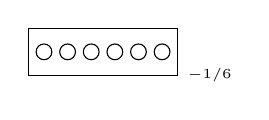
\begin{tikzpicture}
\draw (0, 0) rectangle (1.9, -0.6) node[right]{\tiny $ -1 / 6 $};
\draw (0.2, -0.3) circle (0.1);
\draw (0.5, -0.3) circle (0.1);
\draw (0.8, -0.3) circle (0.1);
\draw (1.1, -0.3) circle (0.1);
\draw (1.4, -0.3) circle (0.1);
\draw (1.7, -0.3) circle (0.1);
\end{tikzpicture}
\qquad
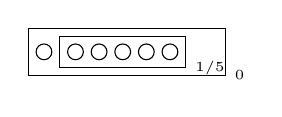
\begin{tikzpicture}
\draw (0, 0) rectangle (2.5, -0.6) node[right]{\tiny $ 0 $};
\draw (0.2, -0.3) circle (0.1);
\draw (0.4, -0.1) rectangle (2, -0.5) node[right]{\tiny $ 1 / 5 $};
\draw (0.6, -0.3) circle (0.1);
\draw (0.9, -0.3) circle (0.1);
\draw (1.2, -0.3) circle (0.1);
\draw (1.5, -0.3) circle (0.1);
\draw (1.8, -0.3) circle (0.1);
\end{tikzpicture}
\qquad
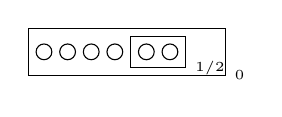
\begin{tikzpicture}
\draw (0, 0) rectangle (2.5, -0.6) node[right]{\tiny $ 0 $};
\draw (0.2, -0.3) circle (0.1);
\draw (0.5, -0.3) circle (0.1);
\draw (0.8, -0.3) circle (0.1);
\draw (1.1, -0.3) circle (0.1);
\draw (1.3, -0.1) rectangle (2, -0.5) node[right]{\tiny $ 1 / 2 $};
\draw (1.5, -0.3) circle (0.1);
\draw (1.8, -0.3) circle (0.1);
\end{tikzpicture}
$$
A simple computation shows that $ \ff(J_X) = (1 / t)^5 \cdot t^4 \cdot (t - 5^5 / 6^6) $.
\end{example}

\end{frame}

\begin{frame}{L-functions}

Let $ k $ be finite, and let $ \rho $ be a nice \footnote{almost everywhere unramified and pure and self-dual of some integral weight} $ \ell $-adic representation of $ F $ for some fixed auxiliary prime $ \ell \ne \ch(k) $. The \textbf{L-function} of $ \rho $ is given by
$$ L(\rho, T) := \prod_{v \in V_F} \det(1 - T \cdot \varphi_v \mid \rho^{I_v})^{-1}, $$
which is the L-function of $ J_X $ when $ \rho = \rho_{J_X} := H_\et^1(\overline{X}, \Q_\ell) $ and $ T = q^{-s} $.

\bigskip

\begin{theorem}[Deligne--Grothendieck]
The numerator of the rational function $ L(\rho, T) $ is precisely $ \det(1 - T \cdot \phi_q \mid H_\et^1(\overline{C}, \FF_\rho)) $ for some constructible sheaves $ \FF_\rho $ on $ C $, and
$$ \dim H_\et^1(\overline{C}, \FF_\rho) = \deg\ff(\rho) + (2g_C - 2)\dim\rho + 2\dim\rho^{\Gal(\overline{k}F / F)}. $$
\end{theorem}

Here, $ \FF_\rho $ is the pushforward of a lisse sheaf on an open subset of $ C $ where $ \rho $ is unramified, and its stalk at any place $ v \in V_F $ is precisely $ \rho^{I_v} $.

\end{frame}

\begin{frame}{Artin formalism}

Let $ K $ be a finite extension of $ F $. Artin's formalism gives a factorisation
$$ L(J_X / K, s) := L(\rho_{J_X / K}, q^{-s}) = \prod_{\chi \in \widehat{G}} L(\rho_{J_X} \otimes \chi, q^{-s}), $$
where $ \widehat{G} $ is the character group of the Galois closure of $ K $ over $ F $.

\bigskip At the level of \'etale cohomology, there are also canonical isomorphisms
$$ H_\et^1(\overline{C}, \FF_{\rho_{J_X / K}}) \cong \bigoplus_{\chi \in \widehat{G}} H_\et^1(\overline{C}, \FF_{\rho_{J_X} \otimes \chi}), $$
which respects the action of $ \phi_q $. Furthermore, if $ \widehat{G} $ can be partitioned into subsets $ o \subseteq \widehat{G} $, then there are canonical isomorphisms
$$ H_\et^1(\overline{C}, \FF_{\rho_{J_X / K}}) \cong \bigoplus_{o \subseteq \widehat{G}} H_\et^1(\overline{C}, \FF_{\rho_{J_X} \otimes (\bigoplus_{\chi \in o} \chi)}). $$

\end{frame}

\begin{frame}{Geometric vanishing}

By Poincar\'e duality, the Tate twist $ H_\et^1(\overline{C}, \FF_{\rho_{J_X}(1) \otimes (\bigoplus_{\chi \in o} \chi)}) $ admits a $ \phi_q $-invariant non-degenerate symmetric bilinear pairing for any $ o \subseteq \widehat{G} $.

\bigskip

\begin{lemma}[Ulmer]
Let $ W_1, \dots, W_{2n} $ be finite-dimensional vector spaces with odd $ \dim W_0 $, and let $ \phi : \bigoplus_{i = 1}^{2n} W_i \to \bigoplus_{i = 1}^{2n} W_i $ be a linear map with $ \phi(W_i) = W_{i + 1} $ for all $ i \in \Z / 2n $, such that $ \bigoplus_{i = 1}^{2n} W_i $ admits a $ \phi_q $-invariant non-degenerate symmetric bilinear pairing that induces an isomorphism $ W_n \cong W_0^* $. Then
$$ 1 - T^{2n} \ \text{divides} \ \det(1 - T \cdot \phi \mid \textstyle\bigoplus_{i = 1}^{2n} W_i). $$
\end{lemma}

In particular, for each subset $ o \subseteq \widehat{G} $ satisfying appropriate assumptions,
$$ 1 - (qT)^{2n} \ \text{divides} \ \det(1 - T \cdot \phi_q \mid H_\et^1(\overline{C}, \FF_{\rho_{J_X} \otimes (\bigoplus_{\chi \in o} \chi)})), $$
which increments the order of vanishing of $ L(J_X / K, s) $.

\end{frame}

\begin{frame}{A Frobenius action}

\begin{example}[Ulmer]
Let $ F = \F_{13}(t) $, and let $ K = \F_{13}(\sqrt[170]{t}) $. Then $ \Gal(\overline{\F_{13}}(t) / \F_{13}(t)) \cong \widehat{\Z} $ is generated by $ \phi_{13} $, which acts naturally on $ \widehat{G} \cong \Z / 170 $ by
$$ \phi_{13}^i \cdot \chi := (\sigma \mapsto \chi(\phi_{13}^i(\sigma))), $$
which translates to multiplication by $ 13^{-1} \equiv -13 \mod 170 $.

\bigskip Let $ \widehat{G} \cong \Z / 170 $ be partitioned by the $ 44 $ orbits of this action given by the singletons $ \{0\} $ and $ \{85\} $, and $ \{\pm n, \pm13n\} $ for each $ n \in \N $.

\bigskip Let $ X $ be as before. If the order of $ \chi \in \widehat{G} $ is sufficiently large,
$$ \dim H_\et^1(\overline{C}, \FF_{\rho_{J_X}(1) \otimes \chi}) \equiv \deg\ff(\rho_{J_X}(1) \otimes \chi) \equiv \deg\ff(\rho_{J_X}) \mod 2, $$
which is odd. Thus the previous lemma applies, and the order of vanishing of $ L(J_X / K, s) $ at $ s = 1 $ is at least $ 44 - c $ for some small $ c \in \N $.
\end{example}

\end{frame}

\begin{frame}{The Birch--Swinnerton-Dyer conjecture}

\begin{conjecture}[Birch--Swinnerton-Dyer]
The order of vanishing of $ L(J_X, s) $ at $ s = 1 $ is $ \rk(J_X) $, with leading term
$$ \lim_{s \to 1} \dfrac{L(J_X, s)}{(s - 1)^{\rk(J_X)}} = \dfrac{\Reg(J_X) \cdot \#\Sha(J_X) \cdot \Tam(J_X)}{\#\tor(J_X)^2}. $$
\end{conjecture}

This implicitly assumes that $ \Sha(J_X) $ is finite, which by the exact sequence
$$ 0 \to J_X(F) \otimes \Z_\ell \to \varprojlim_n \Sel_{\ell^n}(J_X) \to T_\ell\Sha(J_X) \to 0, $$
implies that the first map is an isomorphism.

\bigskip

\begin{theorem}[Artin--Tate, Milne, Schneider, Bauer, Kato--Trihan]
The rank conjecture is equivalent to the finiteness of $ \Sha(J_X)[\ell^\infty] $ for any prime $ \ell $, in which case the leading term conjecture also holds.
\end{theorem}

\end{frame}

\begin{frame}{Invariants of surfaces}

For any nice curve $ X $ over $ F $, there is a unique irreducible proper regular relatively minimal surface $ \XX \to C $ over $ k $, whose generic fibre is $ X $.

\bigskip If $ S $ is a proper regular surface over $ k $, its \textbf{Picard} and \textbf{Brauer groups} are
$$ \Pic(S) := H_\et^1(S, \G_m), \qquad \Br(S) := H_\et^2(S, \G_m). $$
The \textbf{N\'eron--Severi group} $ \NS(S) $ is the image of $ \Pic(S) $ in the quotient of $ \Pic(\overline{S}) $ by its subgroup of divisors algebraically equivalent to zero.

\bigskip

\begin{theorem}[Shioda--Tate]
If $ f_v $ is the number of irreducible components of the fibre $ \XX_v $ at $ v $, then
$$ \rk(\NS(\XX)) - \rk(J_X) = 2 + \sum_v (f_v - 1). $$
\vspace{-0.5cm}
\end{theorem}

\begin{theorem}[Grothendieck]
There is a canonical isomorphism $ \Br(\XX) \xrightarrow{\sim} \Sha(J_X) $.
\end{theorem}

\end{frame}

\begin{frame}{The Tate conjecture}

Analogously to $ J_X $, there is an exact sequence
$$ 0 \to \NS(\XX) \otimes \Z_\ell \xrightarrow{c_\ell} \varprojlim_n H_\et^2(\overline{\XX}, \mu_{\ell^n})^{G_k} \to T_\ell\Br(\XX) \to 0, $$
so the finiteness of $ \Sha(J_X)[\ell^\infty] $ reduces to $ c_\ell $ being an isomorphism.

\bigskip

\begin{conjecture}[Tate]
The cycle class map $ c_\ell $ is an isomorphism for any prime $ \ell $. Equivalently,
$$ \rk(\NS(\XX)) = -\ord_{s = 1} \zeta(\XX, s). $$
\end{conjecture}

In particular, this is independent of $ \ell $. It turns out that
$$ -\ord_{s = 1} \zeta(\XX, s) - \ord_{s = 1} L(J_X, s) = 2 + \sum_v (f_v - 1), $$
so the rank conjecture is equivalent to the Tate conjecture.

\end{frame}

\begin{frame}{A Delsarte surface}

Tate's conjecture is known to hold for rational surfaces, abelian surfaces, elliptic K3 surfaces, and surfaces dominated by a product of nice curves.

\begin{example}[Ulmer]
Let $ X $ be as before. It defines a \emph{Delsarte} surface $ \XX \subseteq \P_{[z : t : x : y]}^3 $ given by
$$ z^4y^2 - x^6 - zx^5 - z^5t = 0, $$
which is dominated by the \emph{Fermat} surface $ S \subseteq \P_{[y_0 : y_1 : y_2 : y_3]}^3 $ given by
$$ y_0^2 + y_1^2 + y_2^2 + y_3^2 = 0, $$
by the rational map $ S \to \XX $ given by
$$ [y_0 : y_1 : y_2 : y_3] \mapsto \left[\dfrac{y_2^{12}}{y_1^{10}} : y_3^2 : \dfrac{y_2^{10}}{y_1^8} : \dfrac{5y_0y_2^6}{y_1^5}\right]. $$
In particular, the Tate conjecture holds for $ \XX $. Thus the rank conjecture, and hence the full Birch--Swinnerton-Dyer conjecture, holds for $ J_X $.
\end{example}

\end{frame}

\begin{frame}{Unbounded ranks}

The previous examples generalise to families of hyperelliptic curves.

\begin{theorem}[Ulmer \footnote{Douglas Ulmer (2007) \emph{L-functions with large analytic rank and abelian varieties with large algebraic rank over function fields}}]
For any $ g, p, r \in \N $ with $ p $ prime, there is a non-isotrivial geometrically irreducible hyperelliptic curves $ X $ of genus $ g $ over $ \F_p(t) $ such that
$$ \ord_{s = 1} L(J_X, s) = \rk(J_X) \ge r. $$
\end{theorem}

For instance, $ X $ could be chosen to be
$$
\begin{cases}
y^2 + xy = x^{2g + 1} + t^{p^n + 1}x & \text{if} \ p = 2, \\
y^2 = x^{2g + 1} + x^{2g} + tx & \text{if} \ 2 < p \mid (2g + 1), \\
y^2 = x^{2g + 2} + x^{2g + 1} + tx & \text{if} \ 2 < p \mid (2g + 2), \\
y^2 = x^{2g + 2} + x^{2g + 1} + t & \text{otherwise}, \\
\end{cases}
$$
in which case $ r \ge (p^n + 1) / 2n - c $ for some $ c \in \N $ independent of $ n $.

\end{frame}

\end{document}